
%### More examples of reflexive, symmetric, transitive
% ### Show relation on R x R using a graph of the subset
%!TEX root = proofs+concepts.tex

\chap{Equivalence Relations and Equivalence Classes}{EquivalenceRelationsChap}

% new command for equivalence class
\newcommand{\class}[1]{\overline{#1}}
\newcommand{\divides}{\mbox{|}}

\medskip\noindent

This can be thought of as a ``pivotal'' chapter. It generalizes the notion of ``function'', and relates this generalization to properties that we discussed in the Modular Arithmetic chapter. We will find that the new concepts we develop in this chapter will be foundational to the notions of \emph{coset} and \emph{conjugate}, two key group-theoretic structures which play central roles in group theory.
\footnote{This chapter  is an adapted and expanded version of a chapter by D. and J. Morris.}

\section{Binary relations} \label{sec.relation}


 Recall that, by definition, any function $f \colon A \to B$ is a set of ordered pairs. More precisely, each element of~$f$ is an ordered pair $(a,b)$, such that $a \in A$ and $b \in B$. Therefore, every element of~$f$ is an element of $A \times B$, so $f$~is a subset of $A \times B$.
\factoidbox{Every function from~$A$ to~$B$ is a subset of $A \times B$.}


\begin{eg} 
The function $\var{mother} \colon \var{PEOPLE} \to \var{PEOPLE}$ is represented by the set
\[ \{\, (p,m)  \in  {\var PEOPLE} \times {\var PEOPLE}  \mid  m  \text{  is the mother of } p \,\} .\]
\end{eg}

\begin{exercise}{student_mother}

\noindent
Let $\var{MY\_GENERATION}$ be the set consisting  of you, your siblings, and any cousins you have.  
\begin{enumerate}[(a)]
\item
List the mothers of all individuals in $\var{MY\_GENERATION}$.
\item
Now for each individual in $\var{MY\_GENERATION}$, write an ordered pair that belongs to the function $\var{mother} \colon \var{PEOPLE} \to \var{PEOPLE}$. (For example, if Ben's  mother is Lucy, then (Ben,Lucy) is an ordered pair that belongs to the function $\var{mother}$.)
\end{enumerate}
\end{exercise}


Many other relationships can also be represented by subsets of $\var{PEOPLE} \times \var{PEOPLE}$, even though they are not functions. For example, $\var{son}$ is not a function, because some people have more than one son (or because some people have no sons at all). However, we can represent this relation by the set
\[  \{\, (p,s) \in  {\var PEOPLE} \times {\var PEOPLE} \mid s \text{ is a son of } p \,\} .\]
	
\begin{exercise}{student_son}
\begin{enumerate}[(a)]
\item
List your parents, siblings, aunts, uncles, and cousins, as a set.  Denote this set as $F$.
\item
Define the relation called $\var{son}$ on $F \times F$ as
\[
\{ (x,y) \in F \times F \,|\, y \text{ is a son of } x \} \]

\noindent
List the ordered pairs in $\var{son}$. (For example, if Paula and Joseph are both in $F$ and Joseph is Paula's son, then (Paula, Joseph) is an ordered pair in $\var{son}$.  Note however if Nathan is in $F$ and Nathan's son Luke is not in $F$, then (Nathan, Luke) is \emph{not} an ordered pair in $\var{son}$.)
\end{enumerate}
\end{exercise}
	
In fact, any relationship that you can define between two people (or, to say this in the official language of logic, any binary predicate on the set $\var{PEOPLE}$) can be represented by an subset of $\var{PEOPLE} \times \var{PEOPLE}$. A few examples of possible relationships are:
	\begin{itemize}
	\item $x$ is a sister of~$y$
	\item $x$ knew $y$ in high school
	\item $x$ is taller than $y$
	\item $x$ and $y$ are in the same math class
	\item etc.
	\end{itemize}
In recognition of this, mathematicians simply \emph{define} a relation to be a set of ordered pairs; that is, a relation is any subset of $A \times B$. Unlike the case of functions, there are no restrictions --- every subset is a relation.


\begin{defn} \label{relation} \index{Relation!definition of} Suppose $A$ and $B$ are sets. 
\begin{enumerate}[(a)]
\item Any subset of $A \times B$ is called a \term{relation from~$A$ to~$B$}.
\item For the special case where $A = B$, any subset of $A \times A$ is called a \term{binary relation} \index{Binary Relation}\index{Relation!binary} on~$A$.
\end{enumerate}
\end{defn}

\begin{eg}\label{ex_rel}
If $A = \{1,2,3\}$ and $B = \{4,5,6\}$, some examples of relations from $A$ to $B$ are:
\[ \{ (1,4), (2,5), (3,6)\}, \]
\[ \{ (1,6), (3,4)\}, \]
\[ \{ (2,5), (3,5) \}, \]
\[ \emptyset, \]
\[ \{ (1,4), (1,5), (1,6), (2,4), (2,5), (2,6), (3,4), (3,5), (3,6) \}.\] 
Notice that all of these sets are subsets of $A \times B$. The final example is the set $A \times B$ itself. Notice that $\emptyset$ is a valid relation because it's a subset of $A \times B$ (a subset with no elements).  On the other hand, the set $\{ \emptyset \}$ is \emph{not} a relation, because it is  a set with one element (namely $\emptyset$), and this element is not an element of $A \times B$. For similar reasons, $\{(1, \emptyset) \}$ is \emph{not} a relation.
\end{eg}

\begin{eg}
Let $A = \{\text{all cities in the U.S.}\}$ and $B = \{\text{all states in the U.S.}\}$. two examples of relations from $A$ to $B$ are:
\[ \{ \text{(Austin,Texas),(Boston,Massachusetts),(Tucson,Arizona)}\}, \]
\[ \{ (x,y) \text{ such that } x \text{ is the capital of } y \}. \]
The first of these relations  is a \emph{subset} of the second.
\end{eg}


\begin{exercise}{7}
\begin{enumerate}[(a)]
\item
Let $A = \{a\}$ and $B = \{1\}$. List \emph{all} relations from $A$ to $B$.
\hyperref[secEqRelChapHints]{(*Hint*)}
\item
Let $A = \{a\}$ and $B = \{1,2\}$. List \emph{all} relations from $A$ to $B$.
\hyperref[secEqRelChapHints]{(*Hint*)}
\item
Let $A = \{a,b\}$ and $B = \{1\}$. List \emph{all} relations from $A$ to $B$.
\hyperref[secEqRelChapHints]{(*Hint*)}
\item
** Let $A = \{a,b\}$. List all the binary relations on $A$.
\hyperref[secEqRelChapHints]{(*Hint*)}
\item
** Let $A = \{a,b,c\}$. How many binary relations are there on the set $A$?
\hyperref[secEqRelChapHints]{(*Hint*)}
\end{enumerate}
\end{exercise}



We will mostly be concerned with binary relations, not relations from some set~$A$ to some other set~$B$.

\begin{eg} 
Some examples of binary relations on $\var{PEOPLE}$ are:
$\var{brother}$, $\var{sister}$, $\var{aunt}$, $\var{uncle}$, $\var{mother}$, $\var{father}$, $\var{grandfather}$, $\var{cousin}$, etc.
 \end{eg}

\begin{defn} \label{digraph} \index{Digraph}
We can draw a picture to represent any given binary relation on any given set~$A$:
	\begin{itemize}
	\item Draw a dot for each element of~$A$.
	\item For $a,b \in A$, draw an arrow from $a$ to~$b$ if and only if $(a,b)$ is an element of the relation.
	\end{itemize} 
The resulting picture is called a \term{digraph}. (The word is pronounced ``DIE-graff'' --- it is short for ``directed graph.''
\end{defn}
 
 \begin{eg}
 Let $A =  \{1,2,3,4,5\}$. We can define a binary relation~$R$ on~$A$ by letting
 	\[ R = \{\, (x,y) \mid x \neq y \text{ and } x^2 + y \leq 10 \,\} .\]
This binary relation is represented by the following digraph:
\\ \centerline{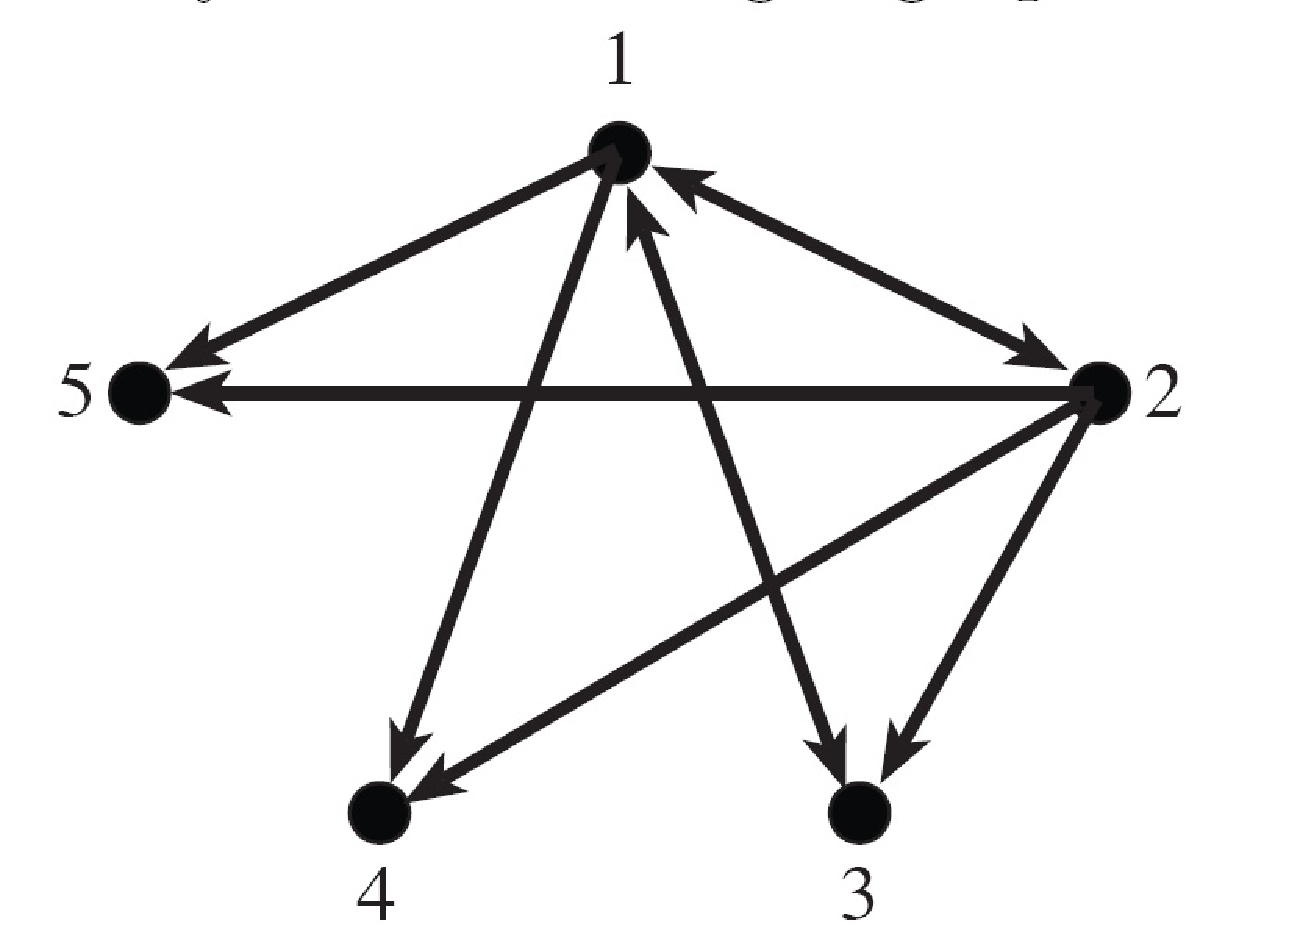
\includegraphics[scale=0.4]{images/x2+y.pdf}}
For example, note that $(x,4) \in R$ iff $x \in \{1,2\}$, and the digraph has arrows from $1$ to~$4$ and from $2$ to~$4$.
\end{eg}

 \begin{exer} \label{DrawBinRelExer}
Using the set $F$ you defined in Exercise~\ref{exercise:EquivalenceRelationsChap:student_son}, draw a digraph for each of the following binary relations on~$F$: 
% In each case, state whether or not your digraph is connected, and whether or not it is strongly connected.
 \begin{enumerate}[(a)]
 \item \label{DrawBinRelExer-son}
 $\var{son}$  (as defined above) 
 \item \label{DrawBinRelExer-sister}
 $\var{sister}$
 \item \label{DrawBinRelExer-married}
 The relation ``has ever been married to."
  \item \label{DrawBinRelExer-lived}
 The relation ``has ever lived with."
 \end{enumerate}
 \end{exer}
 
 \begin{exer} \label{DrawBinRelExer}
Let $A =  \{-2,-1,0,1,2\}$ Draw a digraph for each of the following binary relations on~$A$: 
% In each case, state whether or not your digraph is connected, and whether or not it is strongly connected.
 \begin{enumerate}[(a)]
 \item \label{DrawBinRelExer-son}
 $R_a = \{\, (x,y) \mid  x^2 = y^2 \,\} .$
 \item \label{DrawBinRelExer-sister}
$ R_b = \{\, (x,y) \mid  x^2 - y^2 < 2 \,\} .$
 \item \label{DrawBinRelExer-married}
 $ R_c = \{\, (x,y) \mid  (x-y)^2 < 2 \,\} .$
  \item \label{DrawBinRelExer-lived}
$ R_d = \{\, (x,y) \mid  x\equiv y \pmod{3} \,\} .$
 \end{enumerate}
 \end{exer}

 \begin{exer} \label{DrawBinRelExer2}
It is also possible to draw digraphs for relations that are not binary relations.  
% In each case, state whether or not your digraph is connected, and whether or not it is strongly connected.
 \begin{enumerate}[(a)]
 \item \label{DrawBinRelExer-son}
Draw digraph representations of the relations given in Example \ref{ex_rel}.
 \item \label{DrawBinRelExer-sister}
The graphs you drew in (a) are all examples of \term{bipartite} graphs.  Complete the following definition:  A bipartite graph is a graph in which the vertices (dots) can be divided into two  sets, such that $\ldots \ldots \ldots$.
 \end{enumerate}
 \end{exer}


We commonly use symbols  such as $=, < , \subset, \ldots $  that are used to compare elements of a set. You may have called these ``relations'' in your high school algebra class -- and in fact, they can all be considered as binary relations in the sense of Definition~\ref{relation}.
For example, using the symbol $<$ we can define the following binary relation on ${\mathbb R}$ :
\[ R_<  := \{\, (x,y) \in \mathbb{R} \times \mathbb{R} \mid x < y \}  \]
(here the symbol ``:='' means ``defined as'').  Note that $ R_<$ here is a subset of $\mathbb{R} \times \mathbb{R}$, so it is indeed a binary relation according to Definition~\ref{relation}. 

% This book (like other mathematics textbooks) deals mainly with binary relations on sets of mathematical objects. In fact, you are quite familiar with many relations already. S

\begin{exer} \label{exercise:EquivalenceRelationsChap:RelationDef}
\begin{enumerate}[(a)]
 \item  
 Define the set $R_>$ associated with the symbol ``$>$'' applied to the natural numbers.
 \item  
 Define the set $R_=$ associated with the symbol ``$=$'' applied to the complex numbers. In your definition assume that equality of real numbers has been defined, and write complex numbers in rectangular form (for example, $a + bi$ or $c + di$).
 \item  
 List all the elements of the set $R_\subset$ associated with the symbol ``$\subset$'' applied to the subsets of $A := \{1,2\}$. (The set of subsets of $A$ is denoted as $P(A)$, the \term{power set}\index{Power set} of $A$.)
 \hyperref[secEqRelChapHints]{(*Hint*)}
 \item  
Consider the set $R_\subset$ associated with the symbol ``$\subset$'' applied to the subsets of $A := \{1,2,3\}$. How many elements does $R_\subset$ have?
 \end{enumerate}
 \end{exer}
 
Exercise~\ref{exercise:EquivalenceRelationsChap:RelationDef} shows that any comparison symbol applied to a set gives rise to a binary relation. So rather than writing $R_<, R_>, R_=$ and so on, we simply use the comparison symbol itself to represent the binary relation.  Notice that technically, '$<$' defined on $\mathbb{R}$ is a different relation from '$<$' defined on $\mathbb{N}$: we will always make it very clear which set the relation is being defined on.

We will use the symbol $\rel$ to denote a generic comparison symbol. If we are working with the set $A$, then the symbol $\rel$ also represents the binary relation $A_\rel := \{\, (x,y) \in A \times A \mid x \rel y \}$.

We have shown that comparison symbols give rise to equivalence relations: the reverse is also true. Given a relation $R$ defined on the set $A$, we can define a comparison symbol $\rel$ applied to $a,b \in A$ as follows:
$ a \rel b$ iff $(a,b) \in R$.

There are three basic properties that any given binary relation may or may not have:

\begin{defn} \label{RefSymmTransDefn}
Suppose $\rel$ is a binary relation on a set~$A$. 
\begin{itemize}
\item We say that $\rel$ is \term{reflexive} iff 
	$$ \forall a \in A, a \rel a .$$\index{Relation!reflexive}\index{Reflexive}
In other words, a binary relation on $A$ is reflexive if  every element of A is related to itself.
\item We say that $\rel$ is \term{symmetric} iff 
	$$ \forall a,b \in A,  (a \rel b) \eif (b \rel a)  .$$\index{Relation!symmetric}\index{Symmetric}
In other words, a binary relation on $A$ is symmetric if  whenever $a$ is related to $b$, then $b$ is also related to $a$.  (Here $a$ and $b$ represent elements of the set $A$.)
\item We say that $\rel$ is \term{transitive} iff 
	$$ \forall a,b,c \in A,  \bigl( (a \rel b) \mbox{ and } (b \rel c) \bigr) \eif (a \rel c)  .$$\index{Relation!transitive}\index{Transitive}
In other words, a binary relation on $A$ is transitive if  whenever $a$ is related to $b$ and $b$ is related to $c$, then $a$ is related to $c$.  (Here $a$, $b$ and $c$ represent elements of the set $A$.)
\end{itemize}
\end{defn}

\begin{eg} \ 
Consider the following binary relations on ${\mathbb R}$:
\begin{enumerate}[(a)]
\item $=$ is reflexive, symmetric, and transitive.
\begin{itemize}
\item 
Reflexive:  any real number $x$ equals itself, so $x=x~\forall x \in {\mathbb R}$.
\item
Symmetric:  for any real numbers $x$ and $y$, if $x = y$, then $y = x$. 
\item
Transitive:  for any real numbers $x$, $y$, and $z$, if $x = y$ and $y = z$, then $x = z$.
\end{itemize}
\item $<$ is transitive, but neither reflexive nor symmetric.
\begin{itemize}
\item
Not Reflexive:  For example, it is not true that $1 < 1$.
\item
Not Symmetric:  For example, $1 < 2$ but it is not true that $2 < 1$.
\item
Transitive:  given three real numbers $x$, $y$, and $z$, if $x < y$ and $y < z$, then $x < z$.
\end{itemize}
\item
The binary relation $a \rel b$ iff $a = b + 1$ [for instance $(3.5,2.5) \in {\mathbb R}_\rel$] is neither reflexive, symmetric, or transitive.
\begin{itemize}
\item
Not Reflexive:  $3 \neq 3 + 1$.
\item
Not Symmetric:  $4 \rel 3$, since $4 = 3 + 1$, but $3 \not\rel 4$, since $3 \neq 4 + 1$.
\item
Not Transitive:  $4 \rel 3$ and $3 \rel 2$, but $4 \not\rel 2$ ($4 \neq 2 + 1$).
\end{itemize}  
\end{enumerate}
\end{eg}

Notice that in the above examples, we used specific counterexamples to demonstrate when properties were not true.  We recommend that you do this also, because it is both clear and convincing (and it's usually the easiest way). It only takes \emph{one} counterexample to show a property is not true! 

\begin{exercise}{17}
For each of the following, explain your answers. 
\begin{enumerate}[(a)]
\item Is $\leq$ defined on the set $\mathbb{R}$ transitive? Is it reflexive? Is it symmetric?
\hyperref[secEqRelChapHints]{(*Hint*)}
\item Is $\subset$ defined on the set $P(\mathbb{N})$ transitive? Is it reflexive? Is it symmetric? (Recall that $P(\mathbb{N})$ is the set of subsets of $\mathbb{N}$).
\item Define the relation $\rel$ on $\mathbb{C}$ as follows: $ z_1 \rel z_2$ iff $z_1 = |z_2|$. Is $\rel$ transitive? Is it reflexive? Is it symmetric?
\item Define the relation $\rel$ on $\mathbb{Z}$ as follows: $ a \rel b$ iff $|a - b|< 4$. Is $\rel$ transitive? Is it reflexive? Is it symmetric?
\end{enumerate}
\end{exercise}

%\begin{rem}
%Each of the properties in \cref{RefSymmTransDefn} corresponds to a property of the digraph that we can draw of the relation. 
%\begin{itemize}
%\item A binary relation is reflexive if and only if the corresponding digraph has a loop at every vertex.
%\item A binary relation is symmetric if and only if every arc is in a digon in the corresponding digraph. (In such a case, we generally replace every digon by an edge and model the relation using a graph rather than a digraph.)
%\item A binary relation is transitive if and only if the corresponding digraph has the property that whenever one arc $\vec{uv}$ ends at the start of another arc~$\vec{vw}$, the arc $\vec{uv}$ is also in the digraph.
%\end{itemize}
%\end{rem}

%\begin{exer} \label{SymmTrans->ConnExer}
%Prove that if a binary relation is reflexive, symmetric, and transitive, then the corresponding graph has the property that any two vertices joined by a walk are adjacent. (That is, if there is a walk from~$u$ to~$v$, then $u$ is adjacent to~$v$.  In other words, every connected component of the graph is a complete graph with a loop at every vertex.)
%\hint{Use induction on $n$ to show that if there is a walk of length $n$ from~$u$ to~$v$ in the graph, then the edge $uv$ is in the graph.}
%\end{exer}

%\begin{exers} Suppose $\rel$ is a binary relation on a set~$A$.
%\begin{enumerate}
%\item Show that $\real$ is reflexive iff for all $a \in A$, we have $(a,a) \in \rel$.
%\end{enumerate}
%\end{exers}


\begin{eg}
Given the set $B = \{1,2,3\}$, consider the relation $\rel$ on $B$ defined by 
$$B_\rel = \{(1,1), (2,2), (3,3), (1,2), (2,1), (2,3), (3,2) \}$$
 The relation is shown in the picture below.
 $$ 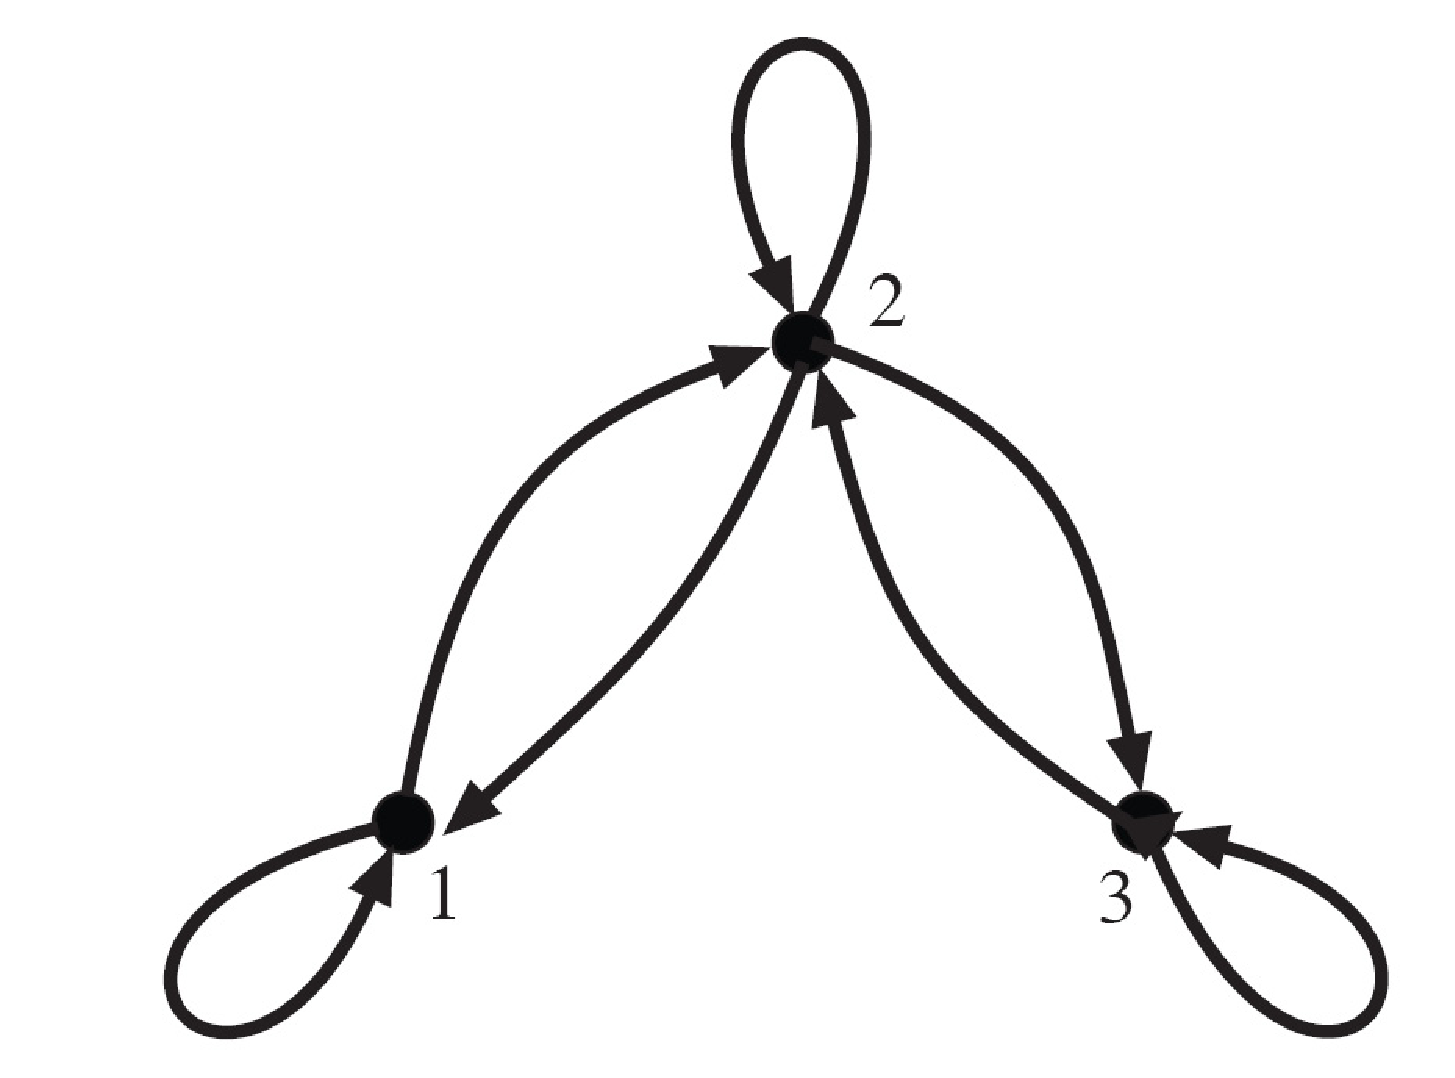
\includegraphics[scale=0.25]{images/GraphRel.pdf} $$
\begin{itemize}
\item $\rel$ is reflexive, because $1 \rel 1$, $2 \rel 2$, and $3 \rel 3$  (Note we had to check \emph{all} elements of the set $B$),
\item $\rel$ is symmetric, because, for each $(a,b) \in \mathord{\rel}$, the reversal $(b,a)$ is also in~$\rel$.
\item $\rel$ is \emph{not} transitive, because $1 \rel 2$ and $2 \rel 3$, but $1 \not\rel 3$.
\end{itemize}
\end{eg}

%
%\begin{eg}
%Let $G$ be a simple graph with edge set $E$.
%Consider the relation $\sim$ defined on the vertex set of $G$ by $u \sim v \eiff uv \in E$.
%This relation:
%\begin{enumerate}
%\item is \emph{not} reflexive, because simple graphs are not allowed to have loops (edges from a vertex to itself);
%\item is symmetric, because if $uv \in E$ then $vu \in E$ is the same edge, looked at from the other end;
%\item may or may not be transitive, depending on the graph $G$.
%\end{enumerate}
%\end{eg}

%
%\begin{eg}
%Let $G$ be a simple digraph with arc set $A$.
%Consider the relation $\sim$ defined on the vertex set of $G$ by $u \sim v \eiff \vec{uv} \in A$.
%This relation:
%\begin{enumerate}
%\item is \emph{not} reflexive, because simple digraphs are not allowed to have loops (arcs from a vertex to itself);
%\item is symmetric only if every arc is part of a digon;
%\item may or may not be transitive, depending on the digraph $G$.
%\end{enumerate}
%\end{eg}

Transitivity can sometimes be a little tricky:

\begin{exercise}{trickyTransitive}
\begin{enumerate}[(a)]
\item
Explain why the binary relation 
\[ R_{\sim} = \{(1,4), (1,1),(4,1) \} \]
is \emph{not} transitive.
\hyperref[secEqRelChapHints]{(*Hint*)} 
\item
Explain why the binary relation 
\[ R_{\sim} = \{(1,2), (1,3),(1,4) \} \]
\emph{is} transitive.
\hyperref[secEqRelChapHints]{(*Hint*)}
\end{enumerate}
\end{exercise}

\begin{exer} \label{BinRelSomePropsEx}
Find binary relations on $\{1,2,3\}$ that meet each of the following conditions 
(Express each relation as a set of ordered pairs, and draw the corresponding digraph.)
\begin{enumerate}[(a)]
\item \label{BinRelSomePropsEx-symmonly}
symmetric, but neither reflexive nor transitive.
\item \label{BinRelSomePropsEx-refonly}
 reflexive, but neither symmetric nor transitive.
\item \label{BinRelSomePropsEx-transandsymm}
transitive and symmetric, but not reflexive.
\item \label{BinRelSomePropsEx-none}
neither reflexive, nor symmetric, nor transitive.
\end{enumerate}
\end{exer}
Digraphs are useful because they represent the relation in such a way that it is easy to deduce the relation's properties: 

\begin{exercise}{21}
\begin{enumerate}[(a)]
\item
How can you tell from looking at a digraph whether or not the corresponding relation is reflexive?
\item
How can you tell from looking at a digraph whether or not the corresponding relation is symmetric? 
\item
**How can you tell from looking at a digraph whether or not the corresponding relation is transitive? (\emph{This one is harder.})
\end{enumerate}
\end{exercise}


%\begin{exer} \label{EvenLengthRelExer}
% \ 
% \begin{enumerate}
%\item \label{EvenLengthRelExer-walk}
% Is the relation ``has a walk of even length" between two vertices of a graph reflexive? symmetric? transitive?  Justify your answers.
%\item \label{EvenLengthRelExer-path}
%  Is the relation ``has a path of even length" between two vertices of a graph reflexive? symmetric? transitive?  Justify your answers.
%\end{enumerate}
%\end{exer}



\section{Definition and basic properties of equivalence relations} \label{EquivalenceRelationsDefnSect}

People often need to sort through a collection of objects, putting similar objects together in a group. 

\begin{eg} \label{EquivRelZooEg}
When making an inventory of the animals in a zoo, we may wish to count the number of antelopes, the number of baboons, the number of cheetahs, and so forth. In this case, all of the animals of the same species might be grouped together. Mathematically speaking, we would define a binary relation $S$ on the set of animals in the zoo by 
\[x \rel_S y \quad \text{iff} \quad x \text{ and } y \text{ are in the same species} .\]
\end{eg}

%When $x$ and~$y$ are placed in the same group (that is, when $x \rel_S y$ in the above example), we may say that $x$ is ``equivalent" to~$y$. This means that $x$ and~$y$ are exactly the same in all respects that are of interest to us. (In the above example, we are interested only in the species of an animal, not its weight, or its age, or anything else.) We call the corresponding binary relation an ``equivalence relation.'' Thus, the binary relation~$\rel_S$ in the above example is an equivalence relation.

Now if we consider the relation $\rel_S$ in light of the properties defined in Definition~\ref{RefSymmTransDefn}, we may discover:
\begin{itemize}
\item  $\rel_S$ is reflexive ($x$ is always the same species as itself);
\item  $\rel_S$ is symmetric ($x$ is the same species as $y$ iff $y$ is the same species as $x$);
\item  $\rel_S$ is transitive (if $x$ is the same species as $y$ and $y$ is the same species as $z$, then $x$ is the same species as $z$);
\end{itemize}

\begin{eg} \label{MoreEquivRelEgs}
\begin{enumerate}[(a)]
\item
If we are concerned only with people's first names, we could define a relation~$\rel_N$ on the set of all people by 
\[  x \rel_N y  \text{~iff~} x \text{ has the same first name as }y.  \]
\item In geometry, sometimes we are interested only in the shape of a triangle and not its location or orientation. In this case, we talk about \emph{congruent} triangles. We may define a relation $\cong$ on the set of all triangles by 
\[T_1 \cong T_2  \text{ iff } T_1  \text{ is congruent  to } T_2. \]
Here ``congruent" means that corresponding sides of the two triangles are equal, and corresponding angles are also equal.
\end{enumerate}
\end{eg}

\begin{exercise}{}
\begin{enumerate}[(a)]
\item
For the relation $\rel_N$ in part (a) of Example~\ref{MoreEquivRelEgs}, explain why it is reflexive, symmetric, and transitive.
\item
For the relation $\cong$ in part (b) of Example~\ref{MoreEquivRelEgs}, explain why it is reflexive, symmetric, and transitive.

%\item For any $n \in \mathbb{N}^+$, \cref{CongEquivRel} tells us  that congruence modulo~$n$ is reflexive, symmetric, and transitive, so it is an equivalence relation on~$\integer$.
\end{enumerate}
\end{exercise}

% In view of the above examples, if $\sim$ is an equivalence relation then we would expect:
% \begin{enumerate}[(a)]
% \item $\sim$ is reflexive ($x$ is the same as~$x$),
% \item $\sim$ is symmetric (if $x$ is the same as~$y$, then $y$ is the same as~$x$),
% and
% \item $\sim$ is transitive (if $x$ is the same as~$y$, and $y$~is the same as~$z$, then $x$~is the same as~$z$).
% \end{enumerate}
The above examples motivate the following definition:

\begin{defn}
An \term{equivalence relation}\index{Equivalence relation} on a set~$A$ is a binary relation on~$A$ that is reflexive, symmetric, and transitive.
\end{defn}

\begin{exer}
\begin{enumerate}[(a)]
\item
``Congruence'' is an equivalence relation on triangles, that you studied in your geometry class. Can you think of another equivalence relation on triangles that you studied in high school geometry?
\item
Define an equivalence relation on the set of all polygons, such that in particular all triangles are equivalent. Explain why your relation is reflexive, symmetric, and transitive. (There are many possible answers to this question.)  
\item
Define an equivalence relation on the set of all polygons, such that in particular not all triangles are equivalent but all rectangles are equivalent. (There are many possible answers to this question.)
\end{enumerate}
\end{exer}

\begin{eg}
Define a binary relation~$\sim$ on~$\real$ by $x \sim y$ iff $x^2 = y^2$. Then $\sim$ is an equivalence relation.

\begin{proof}
We wish to show that $\sim$ is reflexive, symmetric, and transitive.

\noindent
(reflexive) Given $x \in \real $, we have $x^2 = x^2$, so $x \sim x$.

\noindent
(symmetric) Given $x,y \in \real$, such that $x \sim y$, we have $x^2 = y^2$. Since equality is symmetric, this implies $y^2 = x^2$, so $y \sim x$.

\noindent
(transitive) Given $x,y,z \in \real$, such that $x \sim y$ and $y \sim z$, we have $x^2 = y^2$ and $y^2 = z^2$. Therefore $x^2 = z^2$, since equality is transitive. Hence $x \sim z$.
\end{proof}
\end{eg}


%\begin{eg}
%For any $n \in \integer$, we know that congruence modulo~$n$ is reflexive, symmetric, and transitive (see \cref{CongEquivRel}). Therefore, congruence modulo~$n$ is an equivalence relation.
%\end{eg}


\begin{eg} \label{NxNEquivRelEg}
Define a binary relation~$\sim$ on~$\mathbb{N} \times \mathbb{N}$ by $(a_1,b_1) \sim (a_2,b_2)$ iff $a_1 + b_2 = a_2 + b_1$. Then $\sim$ is an equivalence relation.

\begin{proof}
We wish to show that $\sim$ is reflexive, symmetric, and transitive.

\noindent
(reflexive) Given $(a,b) \in \mathbb{N} \times \mathbb{N}$, we have $a + b = a + b$, so $(a,b) \sim (a,b)$.

\noindent
(symmetric) Given $(a_1,b_1) , (a_2,b_2) \in \mathbb{N} \times \mathbb{N}$, such that $(a_1,b_1) \sim (a_2,b_2)$, we have $a_1 +b_2 = a_2 + b_1$. Since equality is symmetric, this implies $a_2 + b_1 = a_1 + b_2$, so $(a_2,b_2) \sim (a_1,b_1)$.

\noindent
(transitive) Given $(a_1,b_1) , (a_2,b_2) , (a_3,b_3) \in \mathbb{N} \times \mathbb{N}$, such that $(a_1,b_1) \sim (a_2,b_2)$ and $(a_2,b_2) \sim (a_3,b_3)$, we have 
\begin{equation} \label{NxNEquivRelEgEqn}
a_1 + b_2 = a_2 + b_1 \text{  and } a_2 + b_3 = a_3 + b_2.
\end{equation}
Therefore 
	\begin{align*}
	(a_1 + b_3) + (a_2 + b_2)
		&= (a_1 + b_2) + (a_2 + b_3) && \text{(rearrange terms)}
		\\&= (a_2 + b_1) + (a_3 + b_2) && \text{(Equation (\ref{NxNEquivRelEgEqn}) above)}
		\\&= (a_3 + b_1) + (a_2 + b_2) && \text{(rearrange terms)} .
	\end{align*}
Subtracting $a_2 + b_2$ from both sides of the equation, we conclude that $a_1 + b_3 = a_3 + b_1$,
so $(a_1,b_1) \sim (a_3,b_3)$.
\end{proof}
\end{eg}


\begin{exercise}{EquivRelShowEx}
Show that each of these binary relations is an equivalence relation.
\begin{enumerate}[(a)]
\item \label{EquivRelShowEx-x2min3x}
The binary relation $\sim$ on $\real$ defined by $x \sim y$ iff $x^2 - 3x = y^2 - 3y$.
\item \label{EquivRelShowEx-xminyinZ}
The binary relation $\sim$ on $\real$ defined by $x \sim y$ iff $x - y \in \integer$.
\hyperref[secEqRelChapHints]{(*Hint*)}
\item \label{EquivRelShowEx-ab=ab}
The binary relation $\sim$ on $\mathbb{N} \times \mathbb{N}$ defined by $(a_1,b_1) \sim (a_2,b_2)$ iff $a_1 b_2 = a_2 b_1$.
\hyperref[secEqRelChapHints]{(*Hint*)}
\item \label{EquivRelComplex1}
The binary relation $\sim$ on $\mathbb{C}$ defined by $z_1 \sim z_2$ iff $|z_1|=|z_2|$.
\item \label{EquivRelComplex1}
The binary relation $\sim$ on $\mathbb{C}$  defined by $z_1 \sim z_2$ iff Re[$z_1$] = Re[$z_2$].  (Recall that Re[$z$] is the real part of $z$)
\item
The binary relation $\sim$ on the collection of all finite sets defined by
\[  A \sim B  \text{ iff } |A|=|B|  \text{  (that is, }A \text{ and } B \text{ have the same number of elements)} \]
\end{enumerate}
\end{exercise}


Any time we have a function, we also get an equivalence relation on its domain:

\begin{eg} \ 
\begin{enumerate}[(a)]
\item Every animal has only one species, so $\var{Species}$ is a function that is defined on the set of all animals. The equivalence relation~$\rel_S$ of Example~\ref{EquivRelZooEg} can be characterized by
\[ x \rel_S y \quad \iff \quad {\var Species}(x) = {\var Species}(y) .\]
\item If we assume that every person has a first name, then $\var{FirstName}$ is a function on the set of all people. The equivalence relation~$\rel_N$ of Example~\ref{MoreEquivRelEgs} can be characterized by
\[  x \rel_N y \quad \iff \quad {\var FirstName}(x) = {\var FirstName}(y) .\]
\end{enumerate}
\end{eg}


The following result generalizes this idea to all functions.

\begin{prop}{EquivRelFromFunc}
Suppose $f \colon A \to B$. If we define a binary relation~$\sim$ on~$A$ by
\[ a_1 \sim a_2 \quad \iff \quad f(a_1) = f(a_2) ,\]
then $\sim$ is an equivalence relation.
\end{prop}

\begin{exercise}{EquivRelFromFuncPfEx}
Prove Proposition~\ref{proposition:EquivalenceRelationsChap:EquivRelFromFunc}. (That is, prove that the relation defined in the proposition is (a) reflexive, (b) symmetric, and (c) transitive.
\end{exercise}



 \section{Equivalence classes} \label{EquivalenceRelationsClassesSect}

If we are interested in first names (as in Example~\ref{MoreEquivRelEgs}), then we may also be interested in the set of all people who have the same first name as you. This is called your ``equivalence class."
 
 \begin{defn}\label{DefEquivRel}
 Suppose $\sim$ is an equivalence relation on a set~$A$. For each $a \in A$, the \term{equivalence class}\index{Equivalence class} of~$a$ is the following subset of~$A$:
 	$$ [a] = \{\, s \in A \mid s \sim a \,\} .$$
That is, the equivalence class of the element $a \in A$ is the set of all elements of $A$ that are equivalent to $a$.
\end{defn}


\begin{eg}
For the equivalence relation~$N$ described in Example~\ref{MoreEquivRelEgs}, we have
	$$ [\var{Alice Cooper}] = \{\, x \in \var{People} \mid \var{FirstName}(x) = \var{FirstName}(\var{Alice Cooper}) \,\} .$$
In other words, $[\var{Alice Cooper}]$ is the set of all people whose first name is Alice.
\end{eg}


\begin{warn}
The notation $[a]$ does not tell us which equivalence relation is being used. You should be able to figure out which relation it is from the context.
\end{warn}


\begin{eg} \label{EquivClassEg}
Suppose $A = \{1,2,3,4,5\}$ and 
\begin{align*}
&R = \\
&\left\{  (1,1), (1,3), (1,4), (2,2), (2,5), (3,1), (3,3), 
		(3,4), (4,1), (4,3), (4,4), (5,2), (5,5) 
\right\}
\end{align*}
One can verify that $R$ is an equivalence relation on~$A$. The equivalence classes are:
$$ [1] = \{1,3,4\},
\quad [2] = \{2,5\} ,
\quad [3] = \{1,3,4\} 
\quad[4] = \{1,3,4\} ,
\quad [5] = \{2,5\} .$$
\end{eg}


\begin{exercise}{EquivClassEasyEx}
\begin{enumerate}[(a)]
\item \label{EquivClassEasyEx-set}
Let $B = \{1,2,3,4,5\}$ and 
	$$S = \left\{ (1,1),\, (1,4),\, (2,2),\, (2,3),\, (3.2),\, 
		(3,3),\, (4,1),\, (4,4),\, (5,5)
		 \right\} .$$
Assume (without proof) that $S$ is an equivalence relation on~$B$. Find the equivalence class of each element of~$B$.


\item \label{EquivClassEasyEx-x+y}
Let $C = \{1,2,3,4,5\}$ and define $\rel_C$ by 
\[ x \rel_C y \iff x + y \text{ is even.} \]
Assume (without proof) that $\rel_C$ is an equivalence relation on~$C$. Find the equivalence class of each element of~$C$.
\item
Draw the arrow diagrams for $\rel_A, \rel_B,$ and $\rel_C$.
\end{enumerate}
\end{exercise}


The following proposition presents some very important properties of equivalence classes:

\begin{thm} \label{EquivRelProps}
Suppose $\sim$ is an equivalence relation on a set~$S$. Then:
\begin{enumerate}[(a)]
\item \label{EquivRelProps-aIn[a]}
 For all $a \in S$, we have $a \in [a]$.
\item \label{EquivRelProps-nonempty}
 For all $a \in S$, we have $[a] \neq \emptyset$.
\item \label{EquivRelProps-union}
 The union of the equivalence classes is all of~$S$. This can be written mathematically as follows:
	$$ \bigcup_{a \in S} [a] = S$$
%Every element of~$S$ is in some equivalence class.
\item \label{EquivRelProps-equal}
 For any $a_1,a_2 \in S$, such that $a_1 \sim a_2$, we have $[a_1] = [a_2]$.
\item \label{EquivRelProps-disjoint}
 For any $a_1,a_2 \in S$, such that $a_1 \not\sim a_2$, we have $[a_1] \cap [a_2] = \emptyset$.
\end{enumerate}
\end{thm}

\begin{exercise}{EquivRelPropsPfEx}
Prove the assertions in Proposition~\ref{EquivRelProps}. You may use the following hints:
\begin{enumerate}[(a)]
\item
Use the reflexive property of $\sim$, together with Definition~\ref{DefEquivRel}
\item
Use part (a).
\item
This can be done by showing:
\begin{enumerate}[(i)]
\item 
$\bigcup_{a \in S} [a] \subset S$
\item
$S \subset \bigcup_{a \in S} [a]$
\end{enumerate}
In (i), use the fact that $[a] \subset S$.  In (ii), use (a) above to show that every element of $S$ is in at least one equivalence class.
\item
Remember that two sets are equal if they have all their elements in common. So you want to show that given $a_1 \rel a_2$, then every element of $[a_1]$ is also an element of [$a_2]$, and vice versa. Do this as follows: 
\begin{itemize}
\item
Choose any $a_3 \in [a_1]$. Use Definition~\ref{DefEquivRel} together with the transitive property to show that $a_3 \in [a_2]$. Conclude that every element of $[a_1]$ is also an element of $[a_2]$. 
\item
Use a similar proof to show that every element of $[a_2]$ is also an element of $[a_1]$.
\end{itemize}
\item
You can prove this one by contradiction. Suppose the intersection is non-empty. Choose an element in the intersection. Use Definition~\ref{DefEquivRel} and the transitive property to derive a contradiction.
\end{enumerate}
\end{exercise}

Proposition~ \ref{EquivRelProps} also gives us this important fact:

\begin{prop}{DisjointEquiv}
Suppose $\sim$ is an equivalence relation on a set~$S$. Then any two equivalence classes are either equal or disjoint; that is, either they have exactly the same elements, or they have no elements in common. 
\end{prop}

\begin{exercise}{DisjointEquivEx}
Fill in the blanks to complete the proof of Proposition~\ref{proposition:EquivalenceRelationsChap:DisjointEquiv}:

\begin{proof}
It's enough to show that any two equivalence classes $[a_1]$ and~$[a_2]$ that are not disjoint must in fact be equal. \index{Disjoint!applied to equivalence relations}
\begin{enumerate}[(a)]
\item
Since the equivalence classes are not disjoint, their intersection is nonempty: so there is some $a \in [a_1] \cap \_\_\_\_\_\_\_\_$. 
\item
Hence, $a \in \_\_\_\_\_\_\_\_$ and $a \in \_\_\_\_\_\_\_\_$. 
\item
By Definition~\ref{DefEquivRel}, this means $a \sim \_\_\_\_\_\_\_\_$ and $a \sim \_\_\_\_\_\_\_\_$. 
\item
Hence, Proposition~\ref{EquivRelProps} part \_\_\_\_\_\_\_\_  tells us that $[a] =\_\_\_\_\_\_\_\_$ and $[a] =\_\_\_\_\_\_\_\_$. 
\item
Therefore $\_\_\_\_\_\_\_\_ = [a] = \_\_\_\_\_\_\_\_$, as desired.
\end{enumerate}
\end{proof}
\end{exercise}


\section{Modular arithmetic redux} \label{EquivalenceRelationsModArithSect}

Abstract algebra often involves looking at familiar concepts and structures in a more general more abstract and ``elegant" way. As an example of this, we will now revisit modular arithmetic and describe it from an entirely different point of view, with the benefit of the concepts we have been developing in previous sections.

In the Modular Arithmetic chapter we defined the concept of ``modular equivalence".  You may recall that we actually gave two definitions, which we repeat here: 

\begin{defn}\label{mod_eqiv_def_1} \emph{(Modular Equivalence, first definition)}

\medskip
$a \equiv b \pmod{n}$ if and only if $a$ and $b$ have the same remainder when divided by $n$.
\end{defn}



\begin{defn}\label{mod_eqiv_def_2} \emph{(Modular Equivalence, second definition)}

\medskip
$a \equiv b \pmod{n}$ iff $a - b = k \cdot n$, where $k$ is an integer (that is, $k \in  {\mathbb Z}$). 
\end{defn}

\begin{exercise}{ProveModEquiv}
Using  Definition  \ref{mod_eqiv_def_2}, show that equivalence mod $n$ is an equivalence relation. (That is, show that equivalence mod $n$ is (a) reflexive, (b) symmetric, and (c) transitive)
\end{exercise}

Exercise~\ref{exercise:EquivalenceRelationsChap:ProveModEquiv} enables us to apply the concepts we've been developing to modular arithmetic. In particular, it enables us to describe modular arithmetic in terms of equivalence classes. We will do this first with a simple example: the integers mod 3.

\subsection{The integers modulo 3}

We have proven in Exercise~\ref{exercise:EquivalenceRelationsChap:ProveModEquiv} that equivalence mod 3 is a bona fide equivalence relation. So what are the equivalence classes? And how many are there?
\medskip

We can use Definition~\ref{mod_eqiv_def_1} to answer this question. The possible remainders when an integer is divided by~$3$ are either $0$, $1$, or~$2$. This tells us that  every integer is equivalent (modulo~$3$) to either $0$, $1$, or~$2$. Using Proposition~\ref{EquivRelProps} part~(d), it follows that:
\begin{itemize}
\item[] for every $k \in \integer$, the equivalence class~$[k]_3$ must be either $[0]_3$, $[1]_3$, or~$[2]_3$.
\end{itemize}
(To emphasize the fact that $n = 3$, we have included a subscript~${}_3$ in the notation for the equivalence classes).

\noindent
Specifically:
\begin{itemize}
\item[]
$[0]_3 = \{ \ldots, -6, -3, 0, 3, 6, \ldots \}$,
\item[]
$[1]_3 = \{ \ldots, -5, -2, 1, 4, 7, \ldots \}$,
\item[]
$[2]_3 = \{ \ldots, -4, -1, 2, 5, 8, \ldots \}$
\end{itemize}
are three equivalence classes that partition the set of all  integers.
In the Modular Arithmetic chapter we defined the integers mod 3\index{Integers mod $n$! as equivalence classes} as the set of remainders under division mod 3. Here we will give an alternative definition that amounts to the same thing:

\begin{defn}\label{mod_eqiv_def_3} \emph{(Integers mod 3, equivalence class definition)}
The set of equivalence classes $\{ [0]_3, [1]_3, [2]_3 \}$ is identified as the set of \term{integers mod 3}, and is represented by the symbol~$\integer_3$.

We may also use the simpler notation $\class{k}$ to represent the equivalence class  $[k]_3$. So we may write either  
$\integer_3 = \{ [0]_3, [1]_3, [2]_3 \}$ or $\integer_3 = \{ \class{0}, \class{1}, \class{2} \} .$
\end{defn}

Notice the subtle (but critically important) difference between this description of modular integers and our previous description. Previously we took the remainders $\{0,1,2\}$ and defined addition and multiplication operations that had the property of closure. But now we are taking a different tack. We are saying that the elements of $\integer_3$ are \emph{equivalence classes} rather than numbers. In other words, the elements of $\integer_3$ are \emph{sets}.

We now define arithmetic operations on $\integer_3$, using our new definition of $\integer_3$ as a set of equivalence classes. Note the additional level of abstraction here: these arithmetic operations are defined on equivalence classes, which are \emph{sets} rather than numbers. But we've seen this before: recall that in the Sets chapter we defined operations on sets. So you're old hands at this!

\begin{defn}\label{RulesOfModArith} (Rules of modular arithmetic)
The \term{arithmetic operations modulo~$3$} are defined as follows:\index{Modular arithmetic!on equivalence classes}
\begin{itemize}
\item $[a]_3 + [b]_3 = [a+b]_3$ \qquad (or $\class{a} + \class{b} = \class{a + b}$),
\item $[a]_3 - [b]_3 = [a-b]_3$ \qquad (or $\class{a} - \class{b} = \class{a - b}$),
\item $[a]_3 \cdot [b]_3 = [ab]_3$ \qquad (or $\class{a} \cdot \class{b} = \class{a  b}$).
\end{itemize}
\end{defn}

In Definition~\ref{RulesOfModArith} we are actually giving \emph{new meanings} to the symbols $+$,$-$, and $\cdot$. We could make this explicit by using different symbols. But this is not really necessary: whenever we're doing arithmetic with equivalence classes mod 3 (or mod $n$, for that matter), you should always presume that we're using the modular definitions of $+$,$-$, and $\cdot$.

\begin{eg}\label{ModPlusExample}
We have $[1]_3 + [2]_3 = [1 + 2]_3 = [3]_3$. However, since 3 and 0 are in the same equivalence class, we have $[3]_3 = [0]_3$, so the above equation can also be written as $[1]_3 + [2]_3 = [0]_3$. Equivalently, $\class{1} + \class{2} = \class{0}$.
\end{eg}

Example~\ref{ModPlusExample} illustrates the following general rule:
$$ \text{%the result of any arithmetic operation (modulo~$3$) will be either $[0]_3$, $[1]_3$, or~$[2]_3$:
 If $r$ is the remainder when $a + b$ is divided by $3$, then $\class{a} + \class{b} = \class{r}$.} $$
You may recognize that this is essentially the same rule that we used in our previous discussion of modular arithmetic.

\begin{exercise}{47}
Write down similar rules for (a) subtraction mod 3; (b) multiplication mod 3.
\end{exercise}

\begin{eg}
Here is a table that shows the results of addition modulo~$3$:
\begin{center} \begin{tabular}{c|c c c}
$+$&$\class{0}$&$\class{1}$&$\class{2}$\\ \hline
$\class{0}$&$\class{0}$&$\class{1}$&$\class{2}$ \\
$\class{1}$&$\class{1}$&$\class{2}$&$\class{0}$ \\
$\class{2}$&$\class{2}$&$\class{0}$&$\class{1}$ \\
\end{tabular}
\end{center}
%\begin{center}
%\begin{tabular}{c||c|c|c}
%$+_3$&$[0]_3$&$[1]_3$&$[2]_3$ \\
%\noalign{\hline}
%\noalign{\smallskip}
%\noalign{\hline}
%$[0]_3$&$[0]_3$&$[1]_3$&$[2]_3$ \\
%\noalign{\hline}
%$[1]_3$&$[1]_3$&$[2]_3$&$[0]_3$ \\
%\noalign{\hline}
%$[2]_3$&$[2]_3$&$[0]_3$&$[1]_3$ \\
%\end{tabular}
%\end{center}
\end{eg}


\begin{exercise}{Mod3TablesEx}
Make tables that show the results of:
\begin{enumerate}[(a)]
\item \label{Mod3TablesEx-multiplication}
multiplication modulo~$3$.
\item \label{Mod3TablesEx-subtraction}
subtraction modulo~$3$ (For $\class{a} - \class{b}$,  put the result in row $\class{a}$ and column; $\class{b}$.)
\end{enumerate}
For both (a) and (b), all table entries should be  either $\class{0}$, $\class{1}$, or $\class{2}$.
\end{exercise}



\subsection{The integers modulo $n$}
The preceding discussion can be generalized to apply with any integer~$n$ in place of~$3$. This results in \term{modular arithmetic}.

\begin{defn} \label{integ_mod_n}
Fix some natural number $n$.
\begin{enumerate}[(a)]
\item For any integer~$k$, we use $[k]_n$ to denote the equivalence class of~$k$ under congruence modulo~$n$. When $n$ is clear from the context, we may write~$\class{k}$, instead of $[k]_n$.
\item The set of these equivalence classes is called the \term{integers modulo~$n$}\index{Integers modulo}. It is denoted~$\integer_n$.

 \item Addition, subtraction, and multiplication modulo~$n$ are defined by:
\begin{itemize}
\item $\class{a} \mathbin{+} \class{b} = \class{a + b}$,
\item $\class{a} \mathbin{-} \class{b} = \class{a - b}$,
and
\item $\class{a} \cdot \class{b} = \class{a  b}$.
\end{itemize}
Just as in the case of mod 3, whenever we're doing arithmetic mod $n$ you should understand that we are using these definitions of  $+$, $-$, and~$\cdot$.
\end{enumerate}
\end{defn}


Note that $\left|\integer_n \right| = n$.\footnote{Recall that for a set $S$, $|S|$ means the number of elements in $S$.} More precisely:

\begin{prop}{}
For any $n \in \mathbb{N}^+$, we have 
	$$\integer_n = \{ \class{0}, \class{1}, \class{2}, \ldots, \class{n-1} \}$$
and $\class{0}, \class{1}, \class{2}, \ldots, \class{n-1}$ are all distinct.
\end{prop}


\begin{exercise}{ModArithEx}  
Make tables that show the results of:
\begin{enumerate}[(a)]
\item \label{ModArithEx-tables-addition} 
addition modulo~$4$.
\item \label{ModArithEx-tables-subtraction} 
subtraction modulo~$5$.
\item \label{ModArithEx-tables-multiplication} 
multiplication modulo~$6$.
\end{enumerate}
\end{exercise}

\begin{exercise}{ModArithEx2}  
Find $x,y \in \integer_{12}$ such that $x \neq \class{0}$ and $y \neq \class{0}$, but $x \cdot y = \class{0}$.
\end{exercise}

\subsection{Something we have swept under the rug} \label{EquivalenceRelationsWellDefSect}

The discussion of modular arithmetic ignored a very important point. When we evaluate $\class{a} \mathbin{+} \class{b}$, we use the following process:
\begin{itemize}
\item
Choose an element from  $\class{a}$ and an element from $\class{b}$;
\item
Add them together (using regular integer arithmetic);
\item
Find the equivalence class of the result. 
\end{itemize}

But suppose we had chosen \emph{different} elements to represent $\class{a}$ and $\class{b}$: how do we know that we would come up with the same answer? In other words: how do we know that $\class{a} \mathbin{+} \class{b}$ is independent of the choice of representatives from $\class{a}$ and $\class{b}$?

So there's a little more work we have to do here to make sure that we don't get into trouble. We need to show that  the operations of addition, subtraction, and multiplication are \term{well-defined}\index{Well defined}: that is, if $a_1, a_2, b_1,$ and $b_2$ are integers such that  $\class{a_1} = \class{a_2}$ and $\class{b_1} = \class{b_2}$, then we need to show that
\begin{enumerate}[(a)]
\item $\class{a_1} \mathbin{+} \class{b_1} = \class{a_2} \mathbin{+} \class{b_2}$,
\item $\class{a_1} \mathbin{-} \class{b_1} = \class{a_2} \mathbin{-} \class{b_2}$, 
\item $\class{a_1} \cdot \class{b_1} = \class{a_2} \cdot \class{b_2}$.
\end{enumerate}
Fortunately, these statements are all true, as you will show in the following exercise.

\begin{exercise}{54} 
\begin{enumerate}[(a)]
\item 
Fill in the blanks in the following proof of statement (a) above that $\mathbin{+}$ is well-defined: 

Suppose $\class{a_1} = \class{a_2}$ and $\class{b_1} = \class{b_2}$. 
\begin{enumerate}[(i)]
\item
From the definition of equivalence class, it follows that  $a_1 \equiv \underline{~<1>~} \pmod{n}$ and $b_1 \equiv \underline{~<2>~} \pmod{n}$. 
\item  
By Definition~\ref{mod_eqiv_def_2}, it follows that 
$a_1 - a_2 = k_1 \cdot \underline{~<3>~}$ and $b_1 - b_2 = k_2 \cdot \underline{~<4>~}$, where $k_1$ and $k_2$ are $\underline{~<5>~}$. 
\item
By integer arithmetic it follows that $(a_1 + b_1) - (a_2 + b_2) =  \underline{~<6>~}$
\item
Since $k_1 + k_2$ is an integer it follows from Definition~\ref{mod_eqiv_def_2} that $(a_1 + b_1) \equiv \underline{~<7>~} \pmod{\underline{~<8>~}}$.
\item 
It follows from Proposition~\ref{EquivRelProps} part (d) that $\underline{~<9>~}$.
\item
By Definition~\ref{integ_mod_n} (c) then $\class{a_1} \mathbin{+} \class{b_1} =  \underline{~<10>~}$; so $\mathbin{+}$ is well-defined.
\end{enumerate}
\item By following the proof in part (a), prove that subtraction mod $n$ is well-defined.
\item By following the proof in part (a), prove that multiplication mod $n$ is well-defined.
\end{enumerate}
\end{exercise}

Actually, finding operations that are well-defined on equivalence classes is somewhat of a big deal. In many cases, candidate operations turn out to be \emph{not} well-defined:

\begin{exercise}{ExpModNotWellDef}
Suppose we try to define an exponentiation operation on $\integer_3$ by:
\[
 {[a]_3}^{\,\wedge} \, [b]_3 = [a^b]_3 \quad \text{ for } [a]_3, [b]_3 \in \integer_3. \]
Show that $\;^{\wedge}$ is not well-defined: that is, find $a, b, c, d \in \integer$, such that $[a]_3 = [c]_3$ and $[b]_3 = [d]_3$, but $\left[a^b \right]_3 \neq \left[c^d \right]_3$.
\end{exercise}

\begin{exercise}{WellDefEx}
\begin{enumerate}[(a)]
\item  \label{WellDefEx-AbsVal0}
 Show that absolute value does \emph{not} provide a well-defined function from~$\integer_7$ to~$\integer_7$. That is, show there exist $a,b \in \integer$, such that 
\[ [a]_7 = [b]_7, \text{ but } \bigl[ |a| \bigr]_7 \neq \bigl[ |b| \bigr]_7.\]
\item  \label{WellDefEx-AbsVal}
 Show that part (a) is true for \emph{every} $n > 2$. That is, show that  absolute value does \emph{not} provide a well-defined function from~$\integer_n$ to~$\integer_n$. 
\end{enumerate}
\end{exercise}

\begin{exercise}{57}
\begin{enumerate}[(a)]
\item
Show that there is a well-defined function 
$f \colon \integer_4 \to \integer_{12}$, given by \\
$ f \bigl( [a]_4 \bigr) = [a]_{12}$. 
That is, show that if $[a]_{12} = [b]_{12}$, then $f \bigl( [a]_4 \bigr) = f \bigl( [b]_4 \bigr)$.
\item  \label{WellDefEx-divide}
Generalize part (a) by showing that if $m$ divides $n$, then there is a well-defined function 
$f \colon \integer_n \to \integer_m$, given by $f \bigl( [a]_n \bigr) = [a]_m$.
That is, show that if $[a]_n = [b]_n$, then $f \bigl( [a]_n \bigr) = f \bigl( [b]_n \bigr)$.
\end{enumerate}
\end{exercise}

\begin{exercise}{}
\begin{enumerate}[(a)]
\item  \label{WellDefEx-odd2}
 Show that if we try to define a function $g \colon \integer_3 \to \integer_2$ by $g \bigl( [a]_3 \bigr) = [a]_2$, then the result is \emph{not} well-defined. That is, show that $\exists a, b \in \integer$ such that
$[a]_3 = [b]_3$  but $[a]_2 \neq [b]_2.$
\item
Generalize part (a) by showing that 
if $m$ does not divide $n$, then the function 
$f: \integer_n \to \integer_m$  given by $f \bigl( [a]_n \bigr) = [a]_m$ is \emph{not} well-defined.
That is, show that there exists integers $a$, $b$ such that $[a]_n = [b]_n$ and $f \bigl( [a]_n \bigr) \neq f \bigl( [b]_n \bigr)$.
\end{enumerate}
\end{exercise}


\section{Partitions}  \label{EquivalenceRelationsPartitionsSect}

Whenever we classify the elements of a particular set, essentially what we are doing is dividing the set up into several disjoint subsets. This is called a  \term{partition}\index{Partition!of a set} of the set. Figure~\ref{partitionfig} below shows a schematic representation of a partition.

\begin{center}
\begin{figure}[ht]
\label{partitionfig}
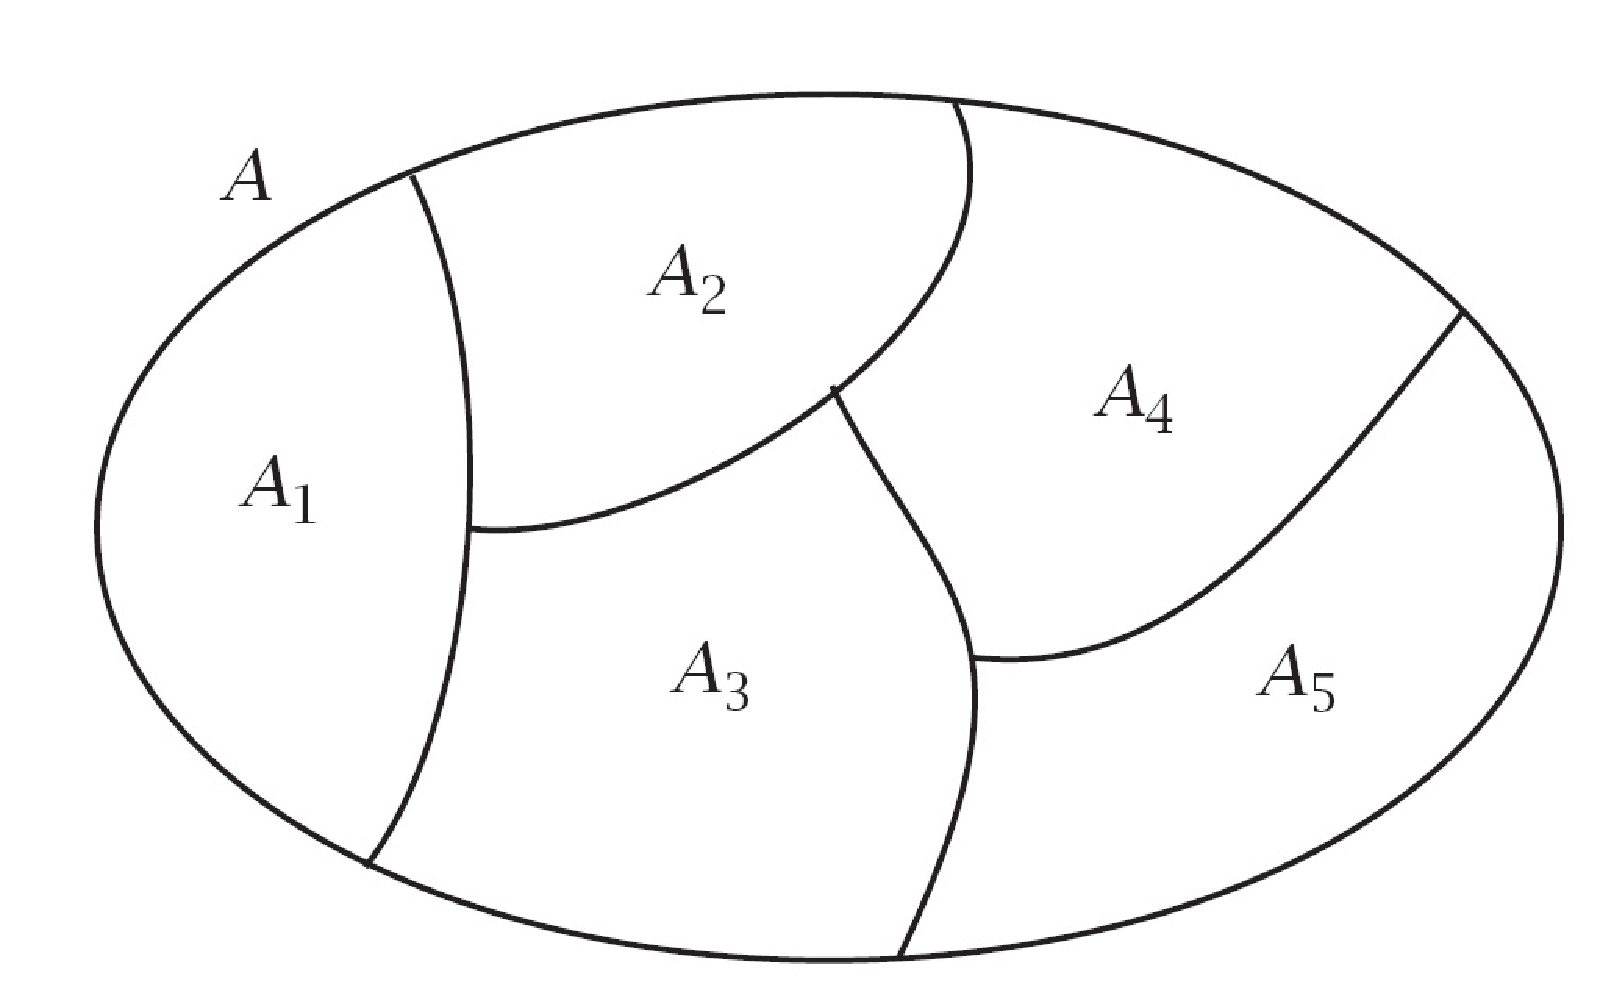
\includegraphics[scale=0.35]{images/partition.pdf}
\caption{A partition of~$A$ into subsets $A_1, \ldots, A_5$. 
(Each element of~$A$ is in one and only one of the subsets.)}
\end{figure}
\end{center}


\begin{eg} \label{ToyPartitionEg}
Mary is leaving for university, and does not want her childhood toys any more, so she will divide them up among her younger siblings: Alice, Bob, and Cindy. Let 
\begin{itemize}
\item $T$ be the set of all of Mary's toys, 
and
\item $A$, $B$, and~$C$ be the set of toys that she will give to Alice, to Bob, and to Cindy, respectively.
\end{itemize}
Then $A$, $B$, and~$C$ are subsets of~$T$, and they should be chosen so that:
\begin{enumerate}[(a)]
\item the union of $A$, $B$ and~$C$ is~$T$ (that is, $A \cup B \cup C = T$), so all of the toys are given away,
and
\item the sets $A$, $B$, and~$C$ are pairwise disjoint (that is, $A \cap B = \emptyset$, $A \cap C = \emptyset$, and $B \cap C = \emptyset$), so there will not be any confusion about who is the new owner of each toy (confusion of ownership among siblings is a dangerous situation).
\end{enumerate}
Here $\{A, B, C\}$ is a  partition of~$T$ into three disjoint subsets (as long as $A, B, C$ are all nonempty). 
\end{eg}
We generalize this example in the following definition:

\begin{defn}
A \term{partition} of a set~$A$ is a collection of nonempty subsets of~$A$, such that each element of~$A$ is in exactly one of the subsets. In other words:
\begin{enumerate}[(a)]
\item the union of the subsets in the collection is all of~$A$,
and
\item the subsets in the collection are pairwise disjoint.\index{Partition!definition of}
\end{enumerate}
\end{defn}


\begin{eg} \label{EquivClassPartEg}
In Example~\ref{EquivClassEg}, the equivalence classes are $\{1,3,4\}$ and $\{2,5\}$. Since $1,2,3,4,5$ each belong to exactly one of these sets, we see that the set
	$$ \bigl\{ \{1,3,4\}, \{2,5\} \bigr\} $$
of equivalence classes is a partition of $\{1,2, 3,4,5\}$.
\end{eg}


The following result is an immediate consequence of Proposition~\ref{EquivRelProps}. It says that equivalence classes always provide a partition.

\begin{thm} \label{EquivRel->Part}
Suppose $\sim$ is an equivalence relation on a set~$A$. Then 
	$$ \{\, [a] \mid a \in A \,\} $$
is a partition of~$A$.
\end{thm}

\begin{proof}
From parts \ref{EquivRelProps-nonempty}, \ref{EquivRelProps-union}, and~\ref{EquivRelProps-disjoint} of Proposition~\ref{EquivRelProps}, we know that the equivalence classes are nonempty, that their union is~$A$, and that they are pairwise disjoint.
\end{proof}

Proposition~\ref{EquivRel->Part} tells us that every equivalence relation gives us a partition\index{Equivalence relation!as a partition}\index{Partition!as an equivalence relation}. Conversely, the following proposition shows that any partition comes from an equivalence relation. In other words, equivalence relations and partitions are just two different ways of looking at the same thing.

\begin{prop}{}\label{Part->EquivRel}
Suppose $\mathcal{P}$ is a partition of a set~$A$. Define a binary relation $\sim$ on~$A$ by
\[ a \sim b \quad \iff \quad \exists C \in \mathcal{P}, ( a \in C \text{ and } b \in C ) .\]
Then:
\begin{enumerate}[(a)]
\item \label{Part->EquivRel-equiv}
 $\sim$ is an equivalence relation on~$A$,
and
\item \label{Part->EquivRel-classes}
 the set of equivalence classes is the partition~$\mathcal{P}$.
\end{enumerate}
\end{prop}



Recall that $\integer_n$ replaces integers $a$ and~$b$ that are congruent modulo~$n$ with objects~$\class{a}$ and~$\class{b}$ that are exactly equal to each other. This was achieved by letting $\integer_n$ be the set of all equivalence classes. The set $\integer_n$ applies only to congruence modulo~$n$, but the same thing can be done for any equivalence relation:

\begin{defn}
Suppose $\sim$ is an equivalence relation on a set~$A$. The set of all equivalence classes is called \term{$A$ modulo~$\sim$}. It is denoted $A/\mathord{\sim}$.
\end{defn}

\begin{eg}
Suppose we define an equivalence relation~$\sim$ on~$\integer$ by $a \sim b$ iff $a \equiv b \pmod{n}$. Then $\integer/\mathord{\sim}$ is simply another name for~$\integer_n$.
\end{eg}

\begin{exercise}{66}
Let $f\colon \{-3,-2,-1,0,1,2,3\} \to \mathbb{N}$ be defined by $f(x) =  x^2$. Define a relation $\sim$ on $\{-3,-2,-1,0,1,2,3\}$ by: $n \sim m$ iff $f(n) = f(m)$.
\begin{enumerate}[(a)]
\item
Show that $\sim$ is an equivalence relation: that is, show that $\sim$ is reflexive, symmetric, and transitive.
\item
According to Proposition~\ref{EquivRel->Part}, this equivalence relation produces a partition on  $\{-3,-2,-1,0,1,2,3\}$. List the sets in the partition.
\end{enumerate}
\end{exercise}

\begin{exercise}{67}
Consider the Cartesian plane $\mathbb{R}^2$. Let $C_r$ be the circle of radius $r$ centered at $(0,0)$, for $r \in [0,\infty)$.(Note that in mathematics, ``circle'' means just the circumference and not the interior: the interior of the circle is called a ``disk''.)
\begin{enumerate}[(a)]
\item
If the point $(x,y) \in C_r$, then write an equation that $(x,y)$ must satisfy.
\hyperref[secEqRelChapHints]{(*Hint*)}
\item
Show that $C_{r}$ and $C_{s}$ are disjoint whenever $r \neq s$. (Do this by showing that any element of $C_{r}$ is not an element of $C_{s}$, and vice versa).
\item
Show that the union of the set of all circles $\{C_r, r \in [0,\infty)$ is all of $\mathbb{R}^2$. (Do this by showing that every element of $\mathbb{R}^2$ is in at least one circle.)
\item
Show that the set of circles centered at $(0,0)$ form a partition of the Cartesian plane.
\hyperref[secEqRelChapHints]{(*Hint*)}
\item
According to Proposition~\ref{Part->EquivRel} part~\ref{Part->EquivRel-equiv}, this partition  defines an equivalence relation $\sim$ on $\mathbb{R}^2$. Use the equation in part (a) of this exercise to complete the following sentence:  $(x_1,y_1) \sim (x_2,y_2)$ iff $\underline{~~~~~~~~~~~~~~}$.
\end{enumerate}
\end{exercise}


%For example, \cref{EquivRel->Part} can be restated as the assertion that if $\sim$ is any equivalence relation on~$A$, then $A/\mathord{\sim}$ is a partition of~$A$.

%% should have some exercises???

%\section{Connected components of a graph}
%???

\begin{summary}
\item Important definitions:
\begin{itemize}
\item relation, binary relation
\item reflexive, symmetric, transitive
\item equivalence relation
\item equivalence class
%\item connected components
\item modular arithmetic
\item integers modulo $n$
\item well-defined
\item partition
\end{itemize}
\item Modular arithmetic is an important example of the use of equivalence classes.
\item Functions must be well-defined.
\item Every binary relation can be drawn as a digraph.
\item Every partition gives rise to an equivalence relation, and vice versa.
\item Notation:
\begin{itemize}
\item $\sim$, $\cong$, or $\equiv$ are used for equivalence relations
\item $[a]$, or $\class{a}$
\item $\integer_n$
\end{itemize}
\end{summary}

 
